% Graphical abstract -- manuscript QTC-2026-07-0055.R1 (IET Quantum Communication)
% Canvas exactly 50 mm x 60 mm (fixed bounding box + clip). One hue (blue ramp),
% Helvetica clone (TeX Gyre Heros), no title, no panel letters (single diagram).
% Text sizes: headings 7 pt bold, details 6.5 pt, results list 6 pt, footer 6 pt.
% The numbers in the results box are the planning-model outputs of the seeded
% synthetic reference scenario (results/summary.csv, figures_src._data.reference()):
% qkd_overlay_links 6 / links_total 35, physical_qkd_hops 13, trusted_sites 7,
% qkd_backed_rekey_pct 94.151 -> 94.2 %, hybrid_premium_5y_npv_kEUR 2838.6 -> 2.84 MEUR.
\documentclass[tikz,border=0pt]{standalone}
\usepackage[T1]{fontenc}
\usepackage{tgheros}
\renewcommand{\familydefault}{\sfdefault}
\usepackage{amsmath}
\usetikzlibrary{arrows.meta,positioning,calc,fit,shapes.misc,backgrounds}
\definecolor{h900}{HTML}{0b2240}\definecolor{h800}{HTML}{14365f}\definecolor{h500}{HTML}{3576bd}\definecolor{h300}{HTML}{86afdb}\definecolor{h100}{HTML}{d6e3f3}\definecolor{h50}{HTML}{edf3fa}\definecolor{ink}{HTML}{1a1a1a}\definecolor{ink2}{HTML}{4a4a4a}\definecolor{ink3}{HTML}{7c7c7c}

% typography helpers
\newcommand{\sep}{\,\textperiodcentered\,}
\newcommand{\hd}[1]{{\fontsize{7}{8.4}\selectfont\bfseries\color{ink}#1}}
\newcommand{\num}[1]{{\bfseries\color{ink}#1}}

\begin{document}
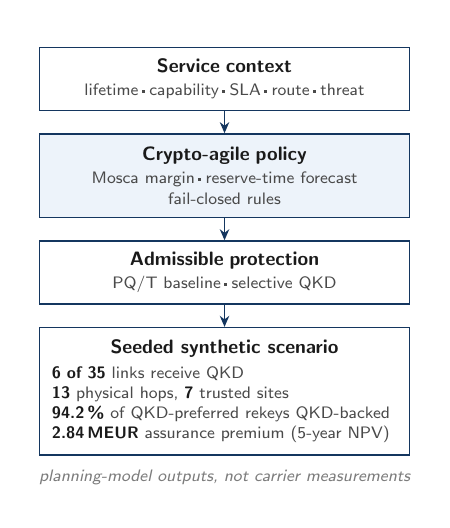
\begin{tikzpicture}[x=1mm,y=1mm,
  % pipeline box: thin dark-blue outline, white fill, centred text
  box/.style={draw=h800, line width=0.5pt, fill=white, anchor=north,
              inner xsep=1.6mm, inner ysep=1.1mm, text width=43.8mm, align=center,
              text=ink2, font=\fontsize{6.5}{7.8}\selectfont},
  % tinted variant for the policy engine (the only tinted element)
  tinted/.style={fill=h50},
  flow/.style={draw=h800, line width=0.5pt, -{Stealth[length=1.4mm,width=1.2mm]}}]
% ---- fixed 50 x 60 mm canvas -------------------------------------------------
\useasboundingbox (0,0) rectangle (50,60);
\clip (0,0) rectangle (50,60);

% ---- tier 1: service context ---------------------------------------------------
\node[box, minimum height=8.0mm] (s1) at (25,57.6)
  {\hd{Service context}\\[0.2ex]
   lifetime\sep capability\sep SLA\sep route\sep threat};

% ---- tier 2: crypto-agile policy (tinted) --------------------------------------
\node[box, tinted, minimum height=10.6mm] (s2) at (25,46.6)
  {\hd{Crypto-agile policy}\\[0.2ex]
   Mosca margin\sep reserve-time forecast\\
   fail-closed rules};

% ---- tier 3: admissible protection ---------------------------------------------
\node[box, minimum height=8.0mm] (s3) at (25,33.0)
  {\hd{Admissible protection}\\[0.2ex]
   PQ/T baseline\sep selective QKD};

% ---- results box ---------------------------------------------------------------
\node[box, minimum height=16.2mm] (res) at (25,22.0) {};
\node[anchor=north, inner sep=0pt, text=ink] at ($(res.north)+(0,-1.6)$)
  {\hd{Seeded synthetic scenario}};
\node[anchor=north west, inner sep=0pt, align=left, text=ink2, text width=43.8mm,
      font=\fontsize{6}{7.3}\selectfont] at ($(res.north west)+(1.6,-5.0)$)
  {\num{6 of 35} links receive QKD\\
   \num{13} physical hops, \num{7} trusted sites\\
   \num{94.2\,\%} of QKD-preferred rekeys QKD-backed\\
   \num{2.84\,MEUR} assurance premium (5-year NPV)};

% ---- flow arrows ---------------------------------------------------------------
\draw[flow] (s1.south) -- (s2.north);
\draw[flow] (s2.south) -- (s3.north);
\draw[flow] (s3.south) -- (res.north);

% ---- footer --------------------------------------------------------------------
\node[anchor=base, inner sep=0pt, text=ink3,
      font=\fontsize{6}{7.2}\selectfont\itshape] at (25,2.4)
  {planning-model outputs, not carrier measurements};
\end{tikzpicture}
\end{document}
